\documentclass[handout, 11pt]{beamer}
\mode
<presentation>{\usetheme{Madrid}}
\institute[UF]{\inst{1}
University of Florida\\
Department of Finance, Insurance, and Real Estate}
\usepackage{adjustbox}
\usepackage{booktabs}
\usepackage{dcolumn}
\newcolumntype{L}[1]{>{\raggedright\let\newline\\\arraybackslash\hspace{0pt}}m{#1}}
\newcolumntype{C}[1]{>{\centering\let\newline\\\arraybackslash\hspace{0pt}}m{#1}}
\newcolumntype{R}[1]{>{\raggedleft\let\newline\\\arraybackslash\hspace{0pt}}m{#1}}
\newcolumntype{.}{D{.}{.}{-1}}
\definecolor{darkgreen}{RGB}{31,156,17}
\usepackage{tikz}
\usetikzlibrary{positioning}
\usetikzlibrary{positioning}
\usetikzlibrary{positioning}
\usetikzlibrary{positioning}
\usetikzlibrary{positioning}
\usetikzlibrary{positioning}
\usepackage{xcolor}
\setbeamertemplate{headline}{\begin{beamercolorbox}[ht=2.25ex, dp=3.75ex]{section in head/foot}
\insertnavigation{\paperwidth}
\end{beamercolorbox}}
\AtBeginSection{\begin{frame}
\frametitle{Table of Contents}
\tableofcontents[currentsection]
\end{frame}}
\begin{document}
\title[Probability]{Probabilistic Modeling}
\subtitle{How to Incorporate Probability into Financial Models}
\author[DeRobertis]{Nick DeRobertis\inst{1}}
\date{\today}
\begin{frame}
\titlepage
\label{title-frame}
\end{frame}
\begin{section}[Intro]{Motivation for Probability Modeling}
\begin{frame}
\frametitle{Why Model Probability}
\begin{columns}
\begin{column}{0.5\textwidth}
\vbox to 0.8\textheight{\begin{itemize}
\item So far everything in our models has been deterministic
\vfill
\item Further, we have not explored any scenarios in our models, we have taken the base case as the only case
\vfill
\item Unfortunately, the real world is very random. Many possible scenarios could occur.
\end{itemize}}
\end{column}
\begin{column}{0.5\textwidth}
\vbox to 0.8\textheight{\centering
\vfill
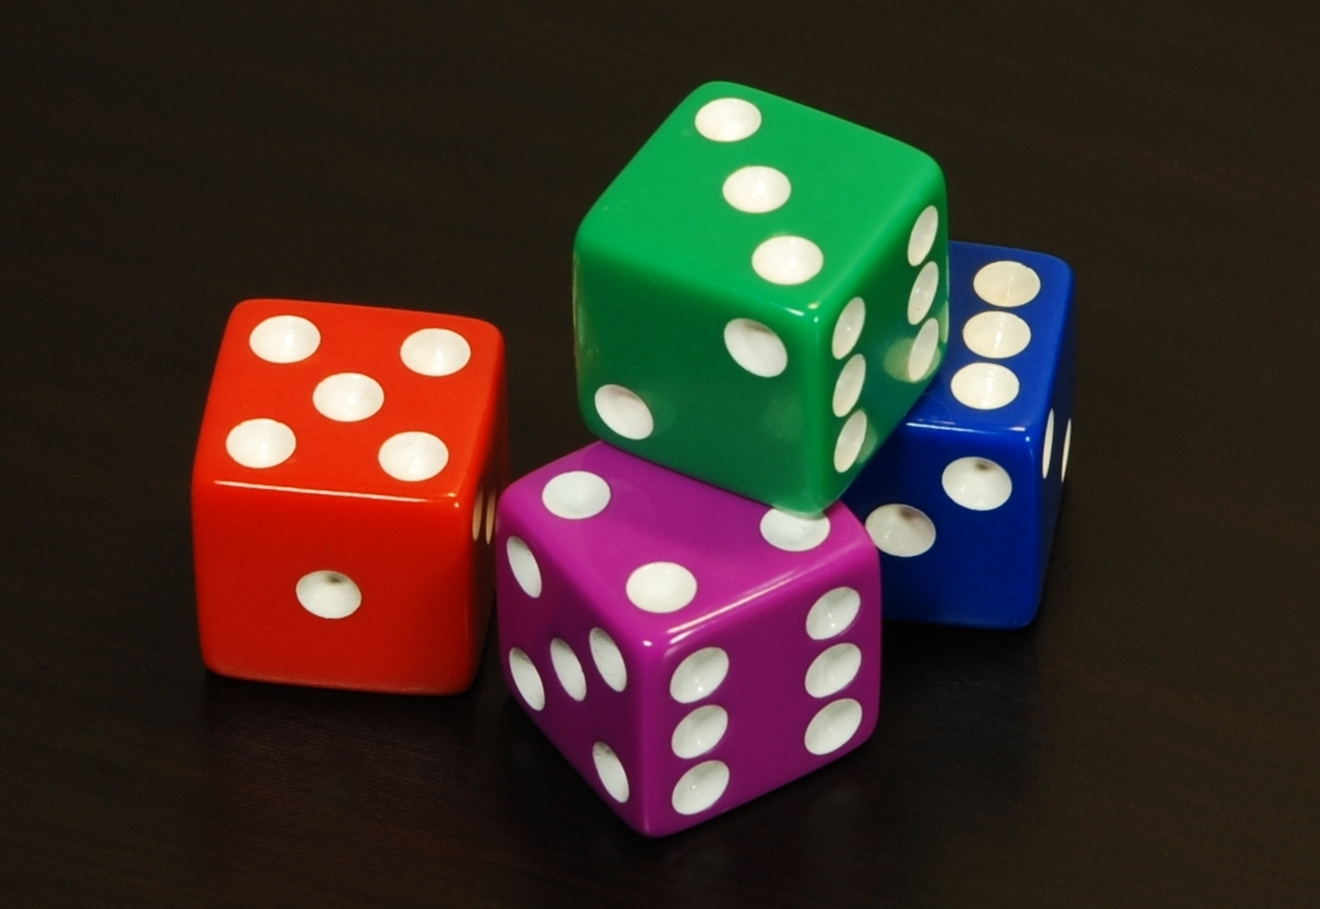
\includegraphics[height=1.0\textheight, keepaspectratio, width=0.9\textwidth]{Sources/dice.jpg}
\vfill
\vfill}
\end{column}
\end{columns}
\end{frame}
\begin{frame}
\frametitle{How to Bring Probability In}
\begin{itemize}
\item There are a few ways we can gain a richer understanding of the modeled situation by incorporating probability
\vfill
\item The simplest is \textbf{scenario modeling}, in which different situations are defined with probabilities, and the result of the model is the expected value across the cases.
\vfill
\item Another is
\textbf{internal randomness}
where randomness is incorporated directly within the model logic
\vfill
\item Finally,
\textbf{Monte Carlo simulation}
treats the model as deterministic but externally varies the inputs to get a distribution of outputs.
\end{itemize}
\end{frame}
\end{section}
\begin{section}[Math Review]{Mathematical Tools for Probability Modeling}
\begin{frame}
\frametitle{Math Review: Discrete and Continuous Variables}
\begin{itemize}
\item When something is measured numerically, it can be either a
\textbf{discrete}
variable, or a
\textbf{continuous}
variable.
\end{itemize}
\begin{block}{Discrete Variables}
\begin{equation}
	x \in \{x_1, x_2, ... x_n\}
\end{equation}
\vspace{-0.4cm}
\begin{itemize}
\item $\{x_1, x_2, ... x_n\}:$
A specific set of values
\end{itemize}
\end{block}
\begin{block}{Continuous Variables}
\begin{equation}
	x \in \mathbb{R} \text{ or } [a, b]
\end{equation}
\vspace{-0.4cm}
\begin{itemize}
\item $\mathbb{R}:$
All real numbers
\item $[a, b]:$
Some interval between two values or infinity
\end{itemize}
\end{block}
\end{frame}
\begin{frame}
\frametitle{Math Review: Expected Value}
\scriptsize
\begin{itemize}
\item \textbf{Expected value}
is the average outcome over repeated trials
\item It is generally useful to get a single output from multiple possible cases
\end{itemize}
\begin{block}{Discrete Variables}
\begin{equation}
	E[x] = \sum_{i=1}^{N} p_i x_i
\end{equation}
\vspace{-0.4cm}
\begin{itemize}
\item $E[x]:$
Expected value for
$x$
\item $x_i:$
A specific value for
$x$
\item $p_i:$
The probability associated with value
$x_i$
\item $N:$
The total number of possible values of
$x$
\end{itemize}
\end{block}
\begin{block}{Continuous Variables}
\begin{equation}
	E[x] = \frac{1}{N} \sum_{i=1}^{N} x_i
\end{equation}
\vspace{-0.4cm}
\begin{itemize}
\item $N:$
The number of samples collected for
$x$
\end{itemize}
\end{block}
\end{frame}
\begin{frame}
\frametitle{Math Review: Variance in One Picture}
\begin{center}
\begin{adjustbox}{width=0.9\textwidth, height=0.8\textheight, keepaspectratio}
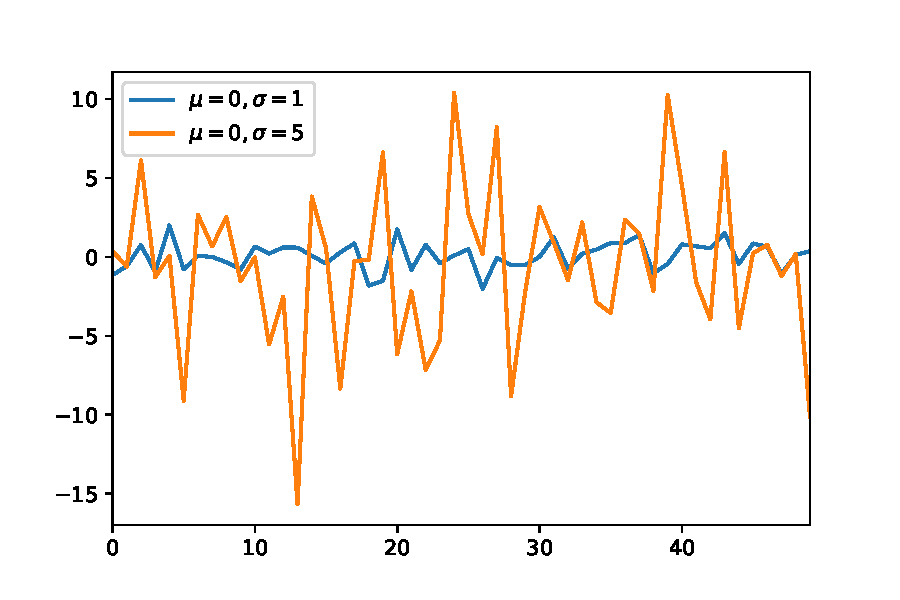
\includegraphics[width=1.0\textwidth]{Sources/different-variance-plot.pdf}
\end{adjustbox}
\end{center}
\end{frame}
\begin{frame}
\frametitle{Math Review: Variance and Standard Deviation}
\footnotesize
\begin{itemize}
\item \textbf{Variance}
and
\textbf{standard deviation}
are measures of the dispersion of values of a random variable.
\item Variance is the real quantity of interest, but standard deviation is easier to understand because it has the same units as the variable, while variance has units squared
\end{itemize}
\begin{block}{Variance of a Continuous Variable}
\begin{equation}
	Var[x] = \sigma^2 = \frac{1}{N - 1} \sum_{i=1}^{N} (x_i - \mu)
\end{equation}
\vspace{-0.3cm}
\begin{itemize}
\item $N:$
Number of samples of
$x$
\item $\mu:$
Sample mean
\end{itemize}
\end{block}
\begin{block}{Standard Deviation}
\begin{equation}
	\sigma = \sqrt{Var[x]}
\end{equation}
\vspace{-0.5cm}
\begin{itemize}
\item $\sigma:$
Standard deviation
\end{itemize}
\end{block}
\end{frame}
\begin{frame}
\frametitle{Math Review: Probability Distributions}
\begin{columns}
\begin{column}{0.5\textwidth}
\vbox to 0.8\textheight{\begin{itemize}
\item A
\textbf{probability distribution}
represents the probabilities of different values of a variable
\vfill
\item For discrete variables, this is simply a mapping of possible values to probabilities, e.g. for a coin toss, heads = 50\% and tails = 50\%
\vfill
\item For continuous variables, a continuous distribution is needed, such as the normal distribution
\end{itemize}}
\end{column}
\begin{column}{0.5\textwidth}
\vbox to 0.8\textheight{\centering
\vfill
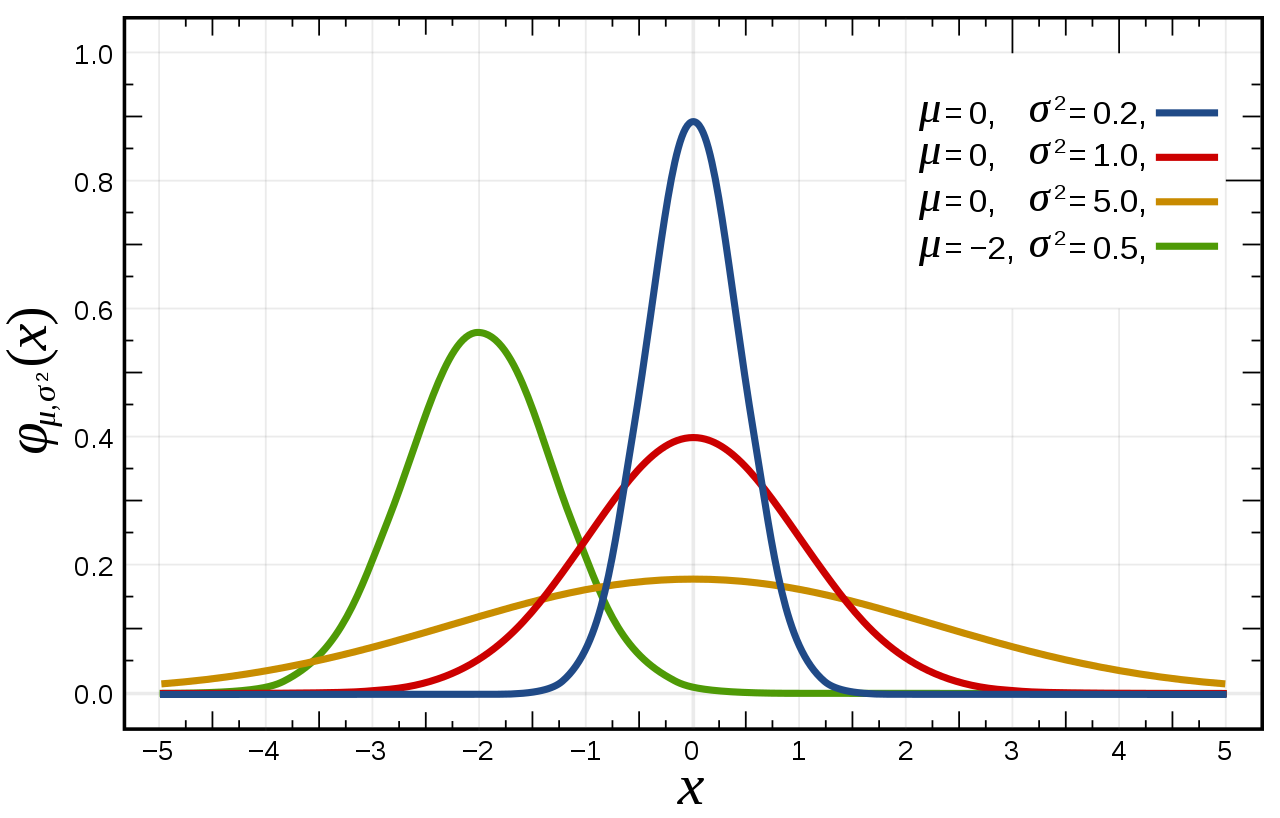
\includegraphics[height=1.0\textheight, keepaspectratio, width=0.9\textwidth]{Sources/normal-distribution.png}
\vfill
\vfill}
\end{column}
\end{columns}
\end{frame}
\begin{frame}
\frametitle{Math Review: Normal Distribution}
\begin{columns}
\begin{column}{0.5\textwidth}
\vbox to 0.8\textheight{\begin{itemize}
\footnotesize
\vfill
\item You've probably heard of the
\textbf{normal distribution}
as it is very commonly used because it occurs a lot in nature
\vfill
\item It is so common because of the
\textbf{central limit theorem}
which says that averages of variables will follow a normal distribution, regardless of the distribution of the variable itself
\vfill
\item This has many applications. For example, we can view the investment rate as an average across individual investment returns, and so it will be normally distributed.
\end{itemize}}
\end{column}
\begin{column}{0.5\textwidth}
\vbox to 0.8\textheight{\centering
\vfill
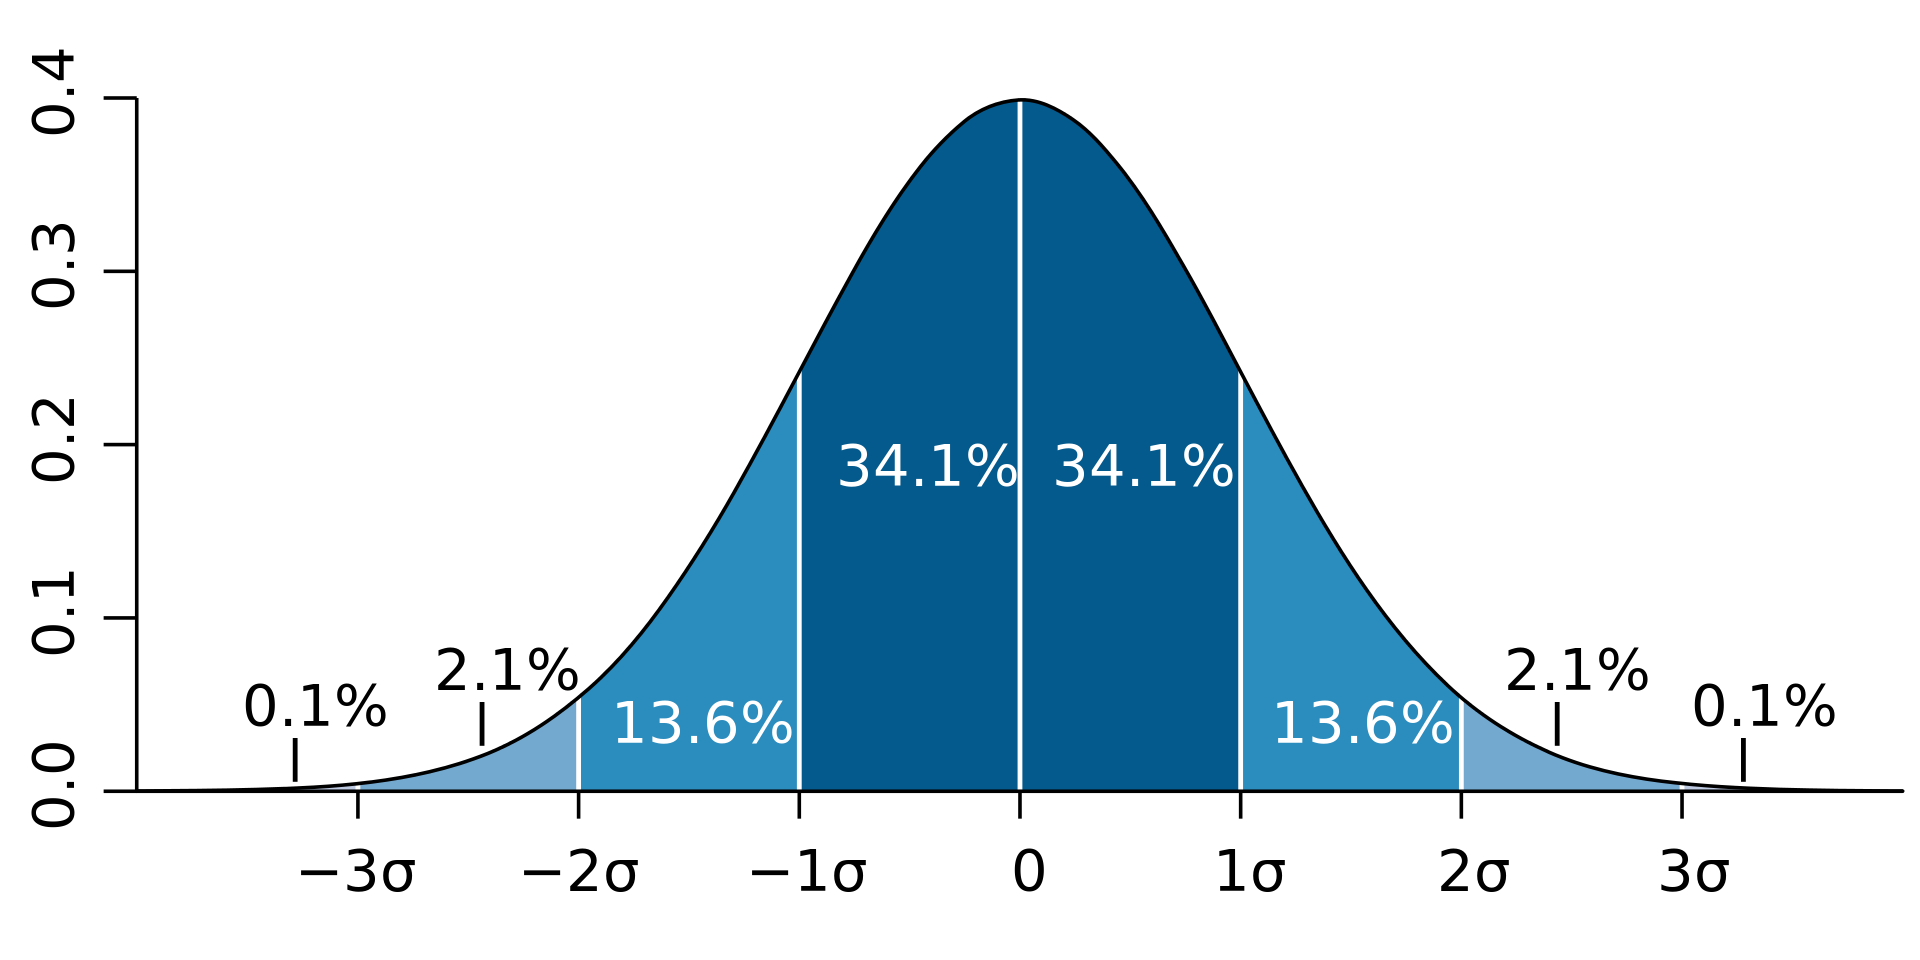
\includegraphics[height=1.0\textheight, keepaspectratio, width=0.9\textwidth]{Sources/normal-distribution-percentages.png}
\vfill
\vfill}
\end{column}
\end{columns}
\end{frame}
\begin{frame}
\frametitle{A Non-Constant Interest Rate}
\scriptsize
\begin{itemize}
\item We want to extend our retirement model to say that the investment return is not constant.
\item We can treat the interest rate as either a discrete (specific values) or a continuous (range of values, more realistic) variable
\end{itemize}
\begin{block}{As a Discrete Variable}
\begin{center}
\begin{tabular}{cc}
Interest Rate & Probability\\

\midrule
2\% & 30\%\\
5\% & 50\%\\
7\% & 20\%\\

\end{tabular}
\end{center}
\end{block}
\begin{block}{As a Continuous Variable}
\begin{equation}
	r_i \sim N(\mu, \sigma^2)
\end{equation}
\vspace{-0.5cm}
\begin{itemize}
\item $N:$
Normal distribution
\item $\mu:$
Interest rate mean
\item $\sigma:$
Interest rate standard deviation
\end{itemize}
\end{block}
\end{frame}
\end{section}
\begin{section}{Scenario Modeling}
\begin{frame}
\frametitle{Scenario Modeling}
\small
\begin{block}{Interest Rate Scenarios}
\begin{center}
\begin{tabular}{l|ccc}
State of Economy & Interest Rate & Savings Rate & Probability\\

\midrule
Recession & 2\% & 35\% & 30\%\\
Normal & 5\% & 30\% & 50\%\\
Expansion & 7\% & 25\% & 20\%\\

\end{tabular}
\end{center}
\end{block}
\begin{itemize}
\item In scenario modeling, different cases for model parameters are chosen. Several parameters may be altered at once in a given case.
\item Here we are making the different cases the state of the economy. When the economy is doing poorly, the individual earns a lower return, but also saves more because they don't want to overspend at a bad time
\item When the economy does well, the individual earns a higher return, but also spends more
\end{itemize}
\end{frame}
\begin{frame}
\frametitle{Implementing Scenario Modeling}
\begin{itemize}
\item We can implement scenario modeling
\textbf{internal}
or
\textbf{external}
to our model
\vfill
\item With an internal implementation, the cases are built
\underline{into the model logic}
itself, and model logic also takes the expected value of the case outputs. The inputs of the model
are now the cases and probabilities.
\vfill
\item With an external implementation, the
\underline{model logic is left unchanged,}
instead the model is run separately with each case, then the expected value is calculated across the outputs from the multiple model runs.
\end{itemize}
\end{frame}
\begin{frame}
\frametitle{Internal or External Scenario Analysis?}
\begin{center}
\begin{tabular}{L{5cm}|R{5cm}}
\textbf{Internal} & \textbf{External}\\

\midrule
\midrule
Original model is now an old version & Original model can still be used normally\\

\midrule
Model runs exactly as before & Getting full results of model requires running the model multiple times and aggregating output\\

\midrule
Model complexity has increased & Model complexity unchanged\\

\midrule
Complexity to run model is unchanged & Complexity to run model has increased\\

\end{tabular}
\end{center}
\end{frame}
\begin{frame}
\frametitle{Scenario Analysis in Excel}
\begin{itemize}
\item For internal scenario analysis, set up a table of the cases and probabilities. Then calculate the expected value of these cases for each model parameter. Then use the expected value as the new model parameter.
\vfill
\item For external scenario analysis, a data table is useful. Create the data table of outputs for each case and another table of case probabilities, then combine them to produce the expected value of the output.
\vfill
\item If you are trying to change more than two inputs at once in external scenario analysis, this becomes more challenging but you can assign a number to each set of inputs and have the model look up the inputs based on the case number, using the case number as the data table input.
\end{itemize}
\end{frame}
\begin{frame}
\frametitle{Scenario Analysis in Excel}
{
\setbeamercolor{block title}{bg=darkgreen}
\begin{block}{Adding Scenario Analysis to the Dynamic Retirement Excel Model}
\begin{itemize}
\item I will now go through adding external scenario analysis to the Dynamic Salary Retirement Model in Excel
\item The completed exercise is in Examples > Scenario Analysis > Excel 
\end{itemize}
\end{block}
}
\end{frame}
\begin{frame}
\frametitle{Scenario Analysis in Excel Lab, Level 1}
{
\setbeamercolor{block title}{bg=violet}
\begin{block}{Adding Scenario Analysis to Project 1, Level 1}
\begin{enumerate}
\item Add external scenario analysis to your Excel model from Project 1
\item Create three cases, for a bad, normal, and good economy. Change the initial demand and price per phone in each of the cases. Both demand and price should be higher in better economic situations. 
\end{enumerate}
\vfill
\end{block}
}
\label{labs:scenario:excel-1}
\end{frame}
\begin{frame}
\frametitle{Scenario Analysis in Python}
\begin{itemize}
\item For internal scenario analysis, set up a
\texttt{DataFrame}
or dictionary of the cases and probabilities. Then calculate the expected value of these cases for each model parameter. Then use the expected value as the new model parameter.
\vfill
\item For external scenario analysis, just call your model function with each input case, collect the results, and combine them to produce the expected value of the output.
\end{itemize}
\end{frame}
\begin{frame}
\frametitle{Scenario Analysis in Python}
{
\setbeamercolor{block title}{bg=darkgreen}
\begin{block}{Adding Scenario Analysis to the Dynamic Retirement Python Model}
\begin{itemize}
\item I will now go through adding external scenario analysis to the Dynamic Salary Retirement Model in Python
\item The completed exercises are in Examples > Scenario Analysis > Python 
\end{itemize}
\end{block}
}
\end{frame}
\begin{frame}
\frametitle{Scenario Analysis in Python Lab, Level 1}
{
\setbeamercolor{block title}{bg=violet}
\begin{block}{Adding Scenario Analysis to Project 1, Level 1}
\begin{enumerate}
\item Add external scenario analysis to your Python model from Project 1
\item Create three cases, for a bad, normal, and good economy. Change the initial demand and price per phone in each of the cases. Both demand and price should be higher in better economic situations. 
\end{enumerate}
\vfill
\end{block}
}
\label{labs:scenario:python-1}
\end{frame}
\end{section}
\begin{section}{Internal Randomness}
\begin{frame}
\frametitle{What is Internal Randomness?}
\begin{itemize}
\item Using the technique of
\textbf{internal randomness,}
something random is added internally to the model
\vfill
\item Instead of taking a fixed input, random values for that variable are drawn
\vfill
\item This technique can be used with both discrete and continuous variables
\end{itemize}
\end{frame}
\begin{frame}
\frametitle{Internal Randomness in One Picture}
\begin{center}
\begin{adjustbox}{width=0.9\textwidth, height=0.8\textheight, keepaspectratio}
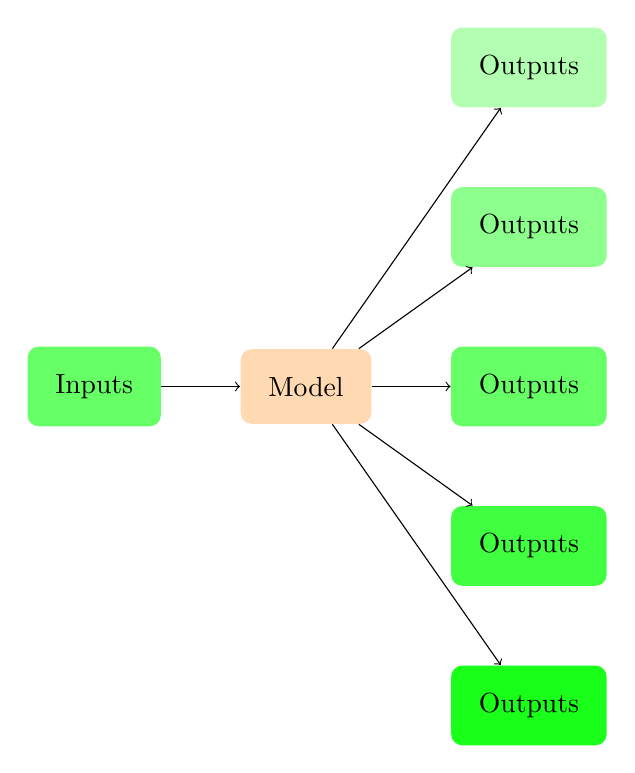
\begin{tikzpicture}
\node [fill=green!30, rounded corners, inner sep=10pt] (c76dabc2-1964-4a10-b72a-88fafa6f2138)  {Outputs};
\node [fill=green!45, rounded corners, inner sep=10pt, below=of c76dabc2-1964-4a10-b72a-88fafa6f2138] (ab3d5dad-7dfb-43ae-aa5d-3acc752e0aad)  {Outputs};
\node [fill=green!60, rounded corners, inner sep=10pt, below=of ab3d5dad-7dfb-43ae-aa5d-3acc752e0aad] (f9bf7c24-76fd-46b5-aab1-e33305c3d589)  {Outputs};
\node [fill=green!75, rounded corners, inner sep=10pt, below=of f9bf7c24-76fd-46b5-aab1-e33305c3d589] (77b7cfc5-f237-4b8b-ade6-b2b41b402949)  {Outputs};
\node [fill=green!90, rounded corners, inner sep=10pt, below=of 77b7cfc5-f237-4b8b-ade6-b2b41b402949] (170050d0-04a2-4a41-8a84-c7c58c1e31e8)  {Outputs};
\node [fill=orange!30, rounded corners, inner sep=10pt, left=of f9bf7c24-76fd-46b5-aab1-e33305c3d589] (4a6151fc-a83a-4b5b-9e7c-e5ffde1e4b60)  {Model};
\node [fill=green!60, rounded corners, inner sep=10pt, left=of 4a6151fc-a83a-4b5b-9e7c-e5ffde1e4b60] (755d7c98-4778-44f2-bbf4-030d2473a6b6)  {Inputs};
\path [draw, ->] (755d7c98-4778-44f2-bbf4-030d2473a6b6) -- (4a6151fc-a83a-4b5b-9e7c-e5ffde1e4b60);
\path [draw, ->] (4a6151fc-a83a-4b5b-9e7c-e5ffde1e4b60) -- (c76dabc2-1964-4a10-b72a-88fafa6f2138);
\path [draw, ->] (4a6151fc-a83a-4b5b-9e7c-e5ffde1e4b60) -- (ab3d5dad-7dfb-43ae-aa5d-3acc752e0aad);
\path [draw, ->] (4a6151fc-a83a-4b5b-9e7c-e5ffde1e4b60) -- (f9bf7c24-76fd-46b5-aab1-e33305c3d589);
\path [draw, ->] (4a6151fc-a83a-4b5b-9e7c-e5ffde1e4b60) -- (77b7cfc5-f237-4b8b-ade6-b2b41b402949);
\path [draw, ->] (4a6151fc-a83a-4b5b-9e7c-e5ffde1e4b60) -- (170050d0-04a2-4a41-8a84-c7c58c1e31e8);
\end{tikzpicture}
\end{adjustbox}
\end{center}
\end{frame}
\begin{frame}
\frametitle{Should I Use Internal Randomness?}
\begin{itemize}
\item Internal randomness makes sense when the random behavior is integral to your model
\vfill
\item If you are just trying to see how changing inputs affects outputs, or trying to get confidence intervals for outputs, an external method such as sensitivity analysis or Monte Carlo simulation would make more sense.
\vfill
\item For example, if we want to allow investment returns to vary in our retirement model, an external method fits well because the core model itself is deterministic
\vfill
\item If instead we were modeling a portfolio, we might use internal randomness to get the returns for each asset.
\end{itemize}
\end{frame}
\begin{frame}
\frametitle{Internal Randomness Advantages and Pitfalls}
\begin{itemize}
\item Similarly to our discussion of internal vs. external sensitivity analysis, internal randomness keeps operational complexity (how to run the model) low, but increases model complexity.
\vfill
\item The main drawback of internal randomness is that the same set of inputs will give different outputs each time the model is run
\vfill
\item While this is the desired behavior, it can make it difficult to determine whether everything is working.
\end{itemize}
\end{frame}
\begin{frame}
\frametitle{Internal Randomness with Continuous Variables}
\begin{columns}
\begin{column}{0.5\textwidth}
\vbox to 0.8\textheight{\begin{itemize}
\item Instead of taking the input as fixed, draw it from a distribution
\vfill
\item We need to define a distribution for each input we want to randomize. This will typically be a normal distribution, and then we just need to give it a reasonable mean and standard deviation
\vfill
\item Put the most reasonable or usual value as the mean. Then think about the probabilities of the normal distribution relative to standard deviation to set it
\end{itemize}}
\end{column}
\begin{column}{0.5\textwidth}
\vbox to 0.8\textheight{\centering
\vfill
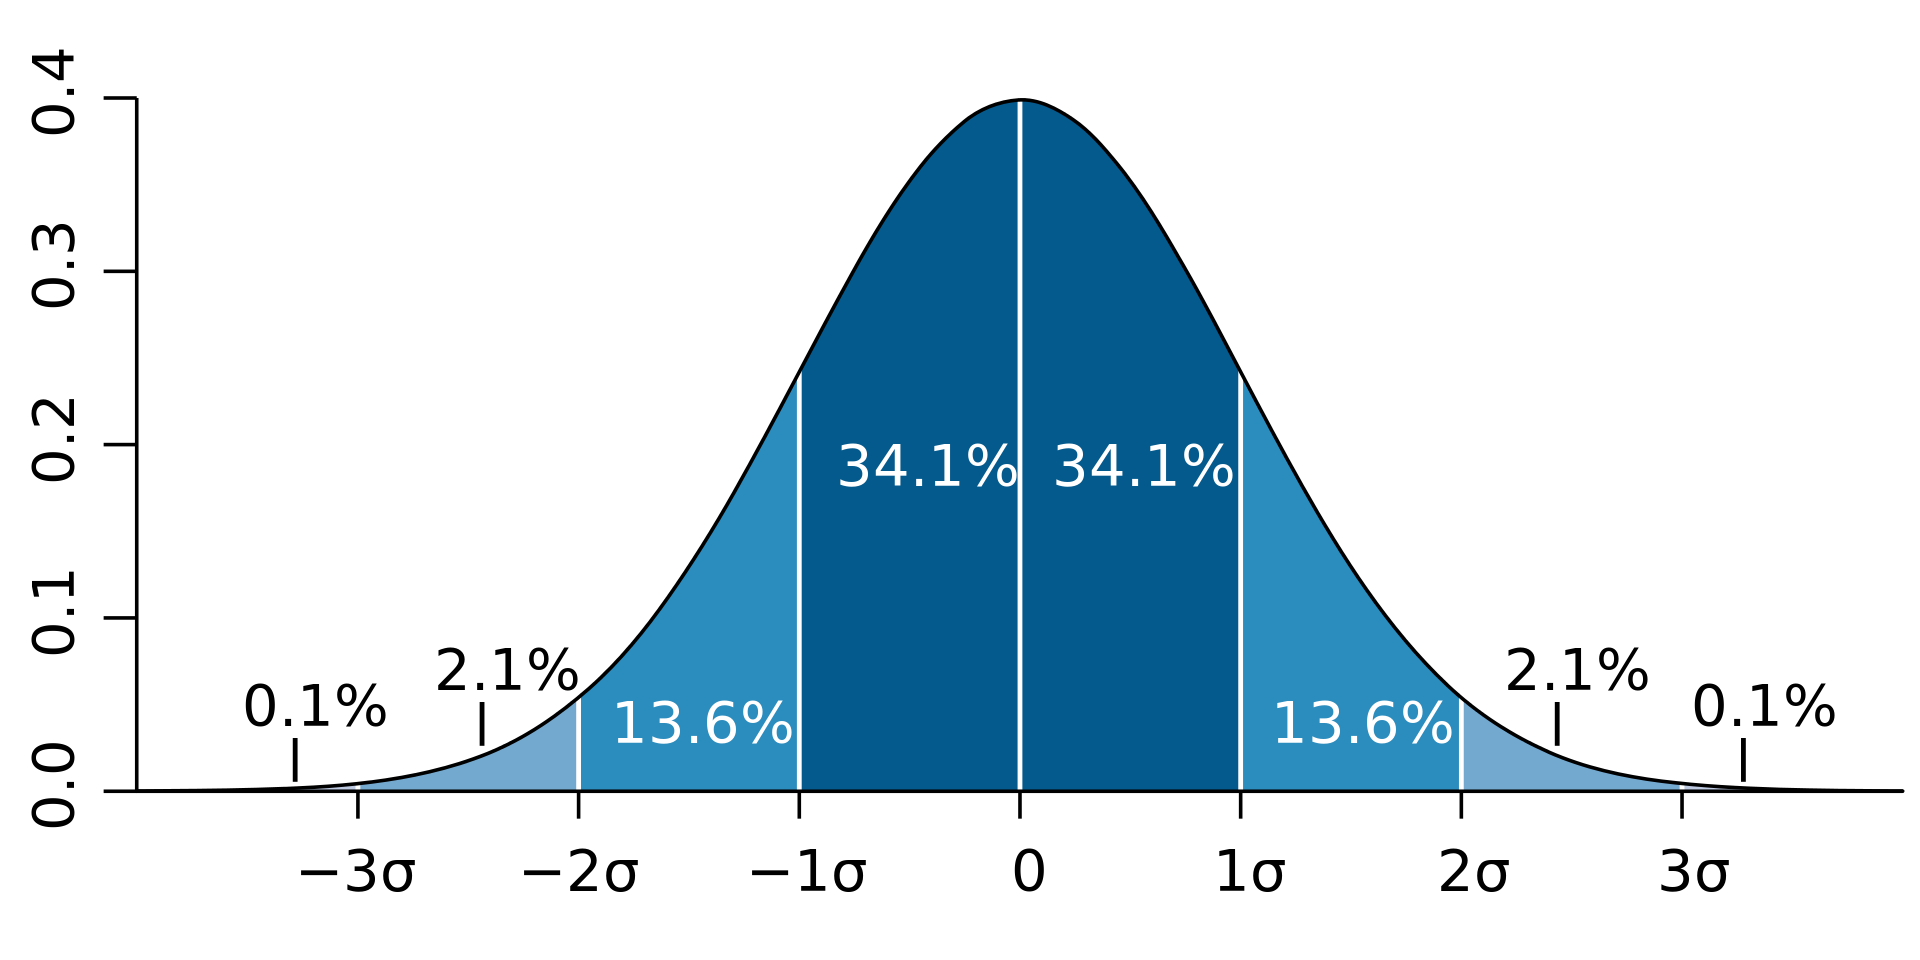
\includegraphics[height=1.0\textheight, keepaspectratio, width=0.9\textwidth]{Sources/normal-distribution-percentages.png}
\vfill
\vfill}
\end{column}
\end{columns}
\end{frame}
\begin{frame}
\frametitle{Internal Randomness with Continuous Variables in Excel}
\begin{itemize}
\item The main functions for randomness in Excel are
\texttt{=RAND}
and
\texttt{=RANDBETWEEN}
\vfill
\item The latter gives a random number between two numbers, while the former gives a random number between 0 and 1. Both of these draw from a uniform distribution (every number equally likely)
\vfill
\item Meanwhile, the
\texttt{=NORM.INV}
function gives the value for a certain normal distribution at a certain probability (it is not random)
\vfill
\item We can combine these two functions to draw random numbers from a normal distribution
\vfill
\item \texttt{=NORM.INV(RAND(), 10, 1)}
would draw a number from a normal distribution with mean 10 and standard deviation 1
\end{itemize}
\end{frame}
\begin{frame}
\frametitle{Example for Continuous Random Variables in Excel}
{
\setbeamercolor{block title}{bg=darkgreen}
\begin{block}{Generating Random Numbers from Normal Distributions in Excel}
\begin{itemize}
\item I will now go through generating random continuous variables in Excel
\item The completed exercise is in Examples > Internal Randomness > Excel 
\item We will focus only on the "Continuous" sheet for now
\end{itemize}
\end{block}
}
\end{frame}
\begin{frame}
\frametitle{Generating and Visualizing Random Numbers in Excel}
{
\setbeamercolor{block title}{bg=violet}
\begin{block}{Getting Started with Randomness in Excel}
Complete the following excercise in Excel for
$n_{iter} = 10$
and
$n_{iter} = 1000$
\begin{itemize}
\item Generate
$n_{iter}$
values between 0 and 1 with a uniform distribution
\item Generate
$n_{iter}$
values from a normal distribution with a 0.5 mean and 10 standard deviation
\item Visualize each of the two outputs with a histogram
\item Calculate the mean and standard deviation of each of the two sets of generated numbers
\item Re-calculate it a few times, take note of how much the mean and standard deviation change
\end{itemize}
\vfill
\end{block}
}
\end{frame}
\begin{frame}
\frametitle{Internal Randomness with Continuous Variables in Python}
\begin{itemize}
\item In Python, we have the built-in
\texttt{random}
module
\vfill
\item It has functions analagous to those in Excel:
\texttt{random.random}
works like
\texttt{=RAND}
and
\texttt{random.uniform}
works like
\texttt{=RANDBETWEEN}
\vfill
\item Drawing numbers from a normal distribution
\textcolor{blue}{\underline{\href{https://docs.python.org/3.7/library/random.html\#real-valued-distributions}{(and other distributions)}}}
is easier: just one function
\texttt{random.normalvariate}
\vfill
\item \texttt{random.normalvariate(10, 1)}
would draw a number from a normal distribution with mean 10 and standard deviation 1
\end{itemize}
\end{frame}
\begin{frame}
\frametitle{Example for Continuous Random Variables in Python}
{
\setbeamercolor{block title}{bg=darkgreen}
\begin{block}{Generating Random Numbers from Normal Distributions in Python}
\begin{itemize}
\item I will now go through generating random continuous variables in Python
\item The completed exercise is in Examples > Internal Randomness > Python 
\item We will focus only on the "Continuous" section for now
\end{itemize}
\end{block}
}
\end{frame}
\begin{frame}
\frametitle{Generating and Visualizing Random Numbers in Python}
\scriptsize
{
\setbeamercolor{block title}{bg=violet}
\begin{block}{Getting Started with Randomness in Python}
Complete the following excercise in Python for
$n_{iter} = 10$
and
$n_{iter} = 1000$
\begin{itemize}
\item Generate
$n_{iter}$
values between 0 and 1 with a uniform distribution
\item Generate
$n_{iter}$
values from a normal distribution with a 0.5 mean and 10 standard deviation
\item Visualize each of the two outputs with a histogram
\item Calculate the mean and standard deviation of each of the two sets of generated numbers
\item Re-calculate it a few times, take note of how much the mean and standard deviation change
\end{itemize}
\vfill
\end{block}
}
\begin{block}{Taking Mean and Standard Deviation in Python}
\begin{itemize}
\item You will likely find it useful to store your data in a
\texttt{DataFrame}
as that makes it easy to calculate mean and standard deviation
\item Once you have your columns in the
\texttt{DataFrame}
just do
\texttt{df.mean()}
to get the mean and
\texttt{df.std()}
to get the standard deviations for each column.
\end{itemize}
\end{block}
\end{frame}
\begin{frame}
\frametitle{Internal Randomness with Discrete Variables}
\begin{itemize}
\item We can also build randomness into the model for discrete variables
\vfill
\item With discrete variables, our distribution is just a table of probabilities for the different values
\vfill
\item To pick a random value for a discrete variable, first add another column to your table which has the cumulative sum of the prior probabilties, and then another column which is that column plus the current probability
\vfill
\item Then generate a random number between 0 and 1 from a uniform distribution
\vfill
\item If the generated number is between the probability and the cumulative sum of prior probabilities, choose that case
\end{itemize}
\end{frame}
\begin{frame}
\frametitle{An Example of Internal Randomness with Discrete Variables}
\small
\begin{block}{Interest Rate Scenarios}
\begin{center}
\begin{tabular}{L{2cm}|cccc}
State of Economy & Interest Rate & Probability & Begin Range & End Range\\

\midrule
Recession & 2\% & 30\% & 0\% & 30\%\\
Normal & 5\% & 50\% & 30\% & 80\%\\
Expansion & 7\% & 20\% & 80\% & 100\%\\

\end{tabular}
\end{center}
\end{block}
\begin{itemize}
\footnotesize
\item The Begin Range column is calculated as the cumulative sum of prior probabilities
\vfill
\item The End Range column is calculated as Begin Range + Probability
\vfill
\item Generate a random number between 0 and 1. If it is between the begin and end range, that is the selected value
\vfill
\item If it's 0.15, it's a recession. If it's 0.45, it's a normal period. If it's 0.94, it's an expansion period.
\end{itemize}
\end{frame}
\begin{frame}
\frametitle{Random Discrete Variables in Python}
\begin{itemize}
\item The steps in the preceeding slides need to be carried out manually in Excel
\vfill
\item In Python, there is a built-in function which is doing all of this in the background,
\texttt{random.choices}
\vfill
\item Simply do
\texttt{random.choices(['Recession', 'Normal', 'Expansion'], [0.3, 0.5, 0.2])}
to yield the exact same result for the prior example
\end{itemize}
\end{frame}
\begin{frame}
\frametitle{Example for Discrete Random Variables in Excel and Python}
{
\setbeamercolor{block title}{bg=darkgreen}
\begin{block}{Generating Random Numbers from Discrete Distributions in Excel and Python}
\begin{itemize}
\item I will now go through generating random discrete variables in both Excel and Python
\item We will be continuing with the same Excel workbook and Jupyter notebook from before which are in Examples > Internal Randomness
\item We will focus only on the "Discrete" sheet/section now
\end{itemize}
\end{block}
}
\end{frame}
\begin{frame}
\frametitle{Example for Discrete Random Variables in Excel and Python}
{
\setbeamercolor{block title}{bg=darkgreen}
\begin{block}{Generating Random Numbers from Discrete Distributions in Excel and Python}
\begin{itemize}
\item I will now add internal randomness with discrete variables to both the Excel and Python Dynamic Salary Retirement models to simulate economic conditions changing year by year
\item The completed models are in Examples > Internal Randomness
\item We will focus only on the "Discrete" sheet/section now
\end{itemize}
\end{block}
}
\end{frame}
\begin{frame}
\frametitle{Random Discrete Variables in Python and Excel}
{
\setbeamercolor{block title}{bg=violet}
\begin{block}{A Simple Model of a Stock Price Over Time}
\begin{itemize}
\item A stock starts out priced at 100. Each period, it can either go up or down.
\item When it goes up, it will grow by 1\%. When it goes down, it will decrease by 1\%.
\item The likelihood of the stock going up is 60\%, and down 40\%.
\item Build a model which shows how the stock price changes throughout time. Visualize it up to 100 periods and show the final price.
\end{itemize}
\vfill
\end{block}
}
\end{frame}
\end{section}
\end{document}